\section{Análisis de los resultados}

En esta sección vamos a analizar los resultados obtenidos en la simulación, centrándonos principalmente en las diferentes anchuras de la energía de excitación recostruida. Dado que tendremos dos anchuras, en función de la energía de excitación vamos a usar la notación $\sigma(E^*)$ como anchura del ajuste gaussiano a la distribución de energía de excitación recostruida para $E^*$.  

\subsection{Recostrucción sin fuentes de incertidumbre}

En primer lugar vamos a analizar la recostrucción de la energía de excitación sin considerar ninguna fuente de incertidumbre de las aquí modeladas, que como ya mencionamos son el sttragling, la dispersión angular y la resolución de los silicios. Como podemos ver en la imagen \cref{Fig:05-RecExcIdx3}, obtenemos prácticamente una distribución Briet-Wigner, con 

\begin{equation}
    \sigma_{0} (0) = \num{0.001363305730(0.0000960943)} \text{ MeV} \quad 
    \sigma_{0} (0.2) = \num{0.011362236853(0.0034089820)} \text{ MeV}
\end{equation} 
el origen de esta $\sigma$ se puede deber al cálculo numérico del ordenador, ya que entre interacción e interacción se pierden dígitos, posibles errores sistemáticos en la simulación, e incluso errores en la generación de las distribuciones de los parámetros iniciales (energía de excitación, punto de interacción...). En cualquier caso, un análisis máx exahustivo del error permitiría obtener un origen claro de esta $\sigma$, y sería una buena práctica para futuras simulaciones.

\vspace*{-0.25cm}
\begin{figure}[H]
    \centering
    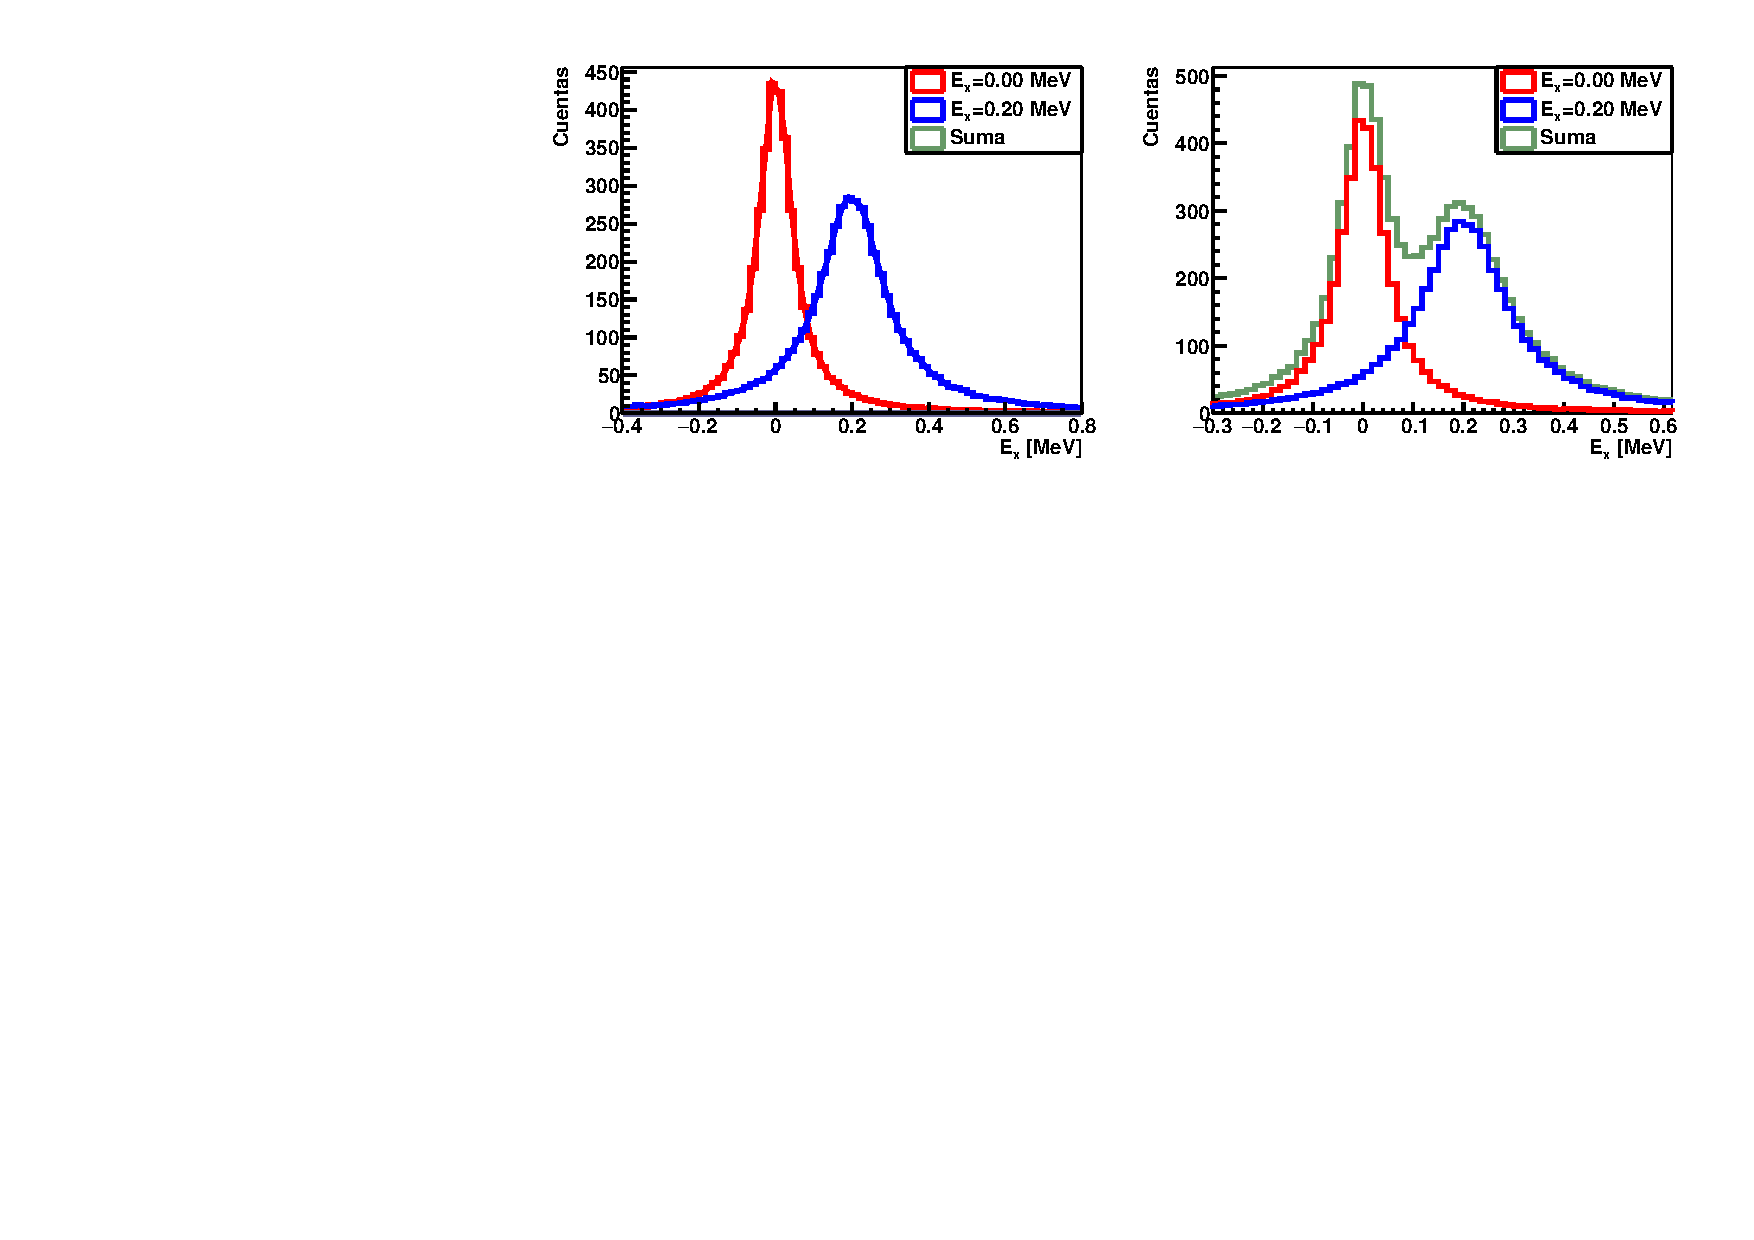
\includegraphics[width=0.9\textwidth]{Imagenes/Rec_incIdx3_single.pdf}
    \caption{Energía de excitación sin incertidumbre.}
    \label{Fig:05-RecExcIdx3}
\end{figure}

En cualquier caso, podemos ver claramente que la anchura intríseca de los estados del litio 10 ya produce un efecto de superposición de picos que dificultará el tratamiendo de datos experimentales, incluso reduciendo errores sistemáticos y estadísticos.

Cada una de las $\sigma$ obtenidas estarán afectadas por este error, tal que en realidad la $\sigma$ que podemos inferir de la simulación será:
\begin{equation}
    \sigma_{real}^2 = \sigma_{obtenida}^2 - \sigma_{0}^2
\end{equation}
Aunque como podemos ver en  \cref{Tab:05-ExcRec} la $\sigma_{0}$ es muy pequeña comparándola con lo obtenido en los otras simulaciones, por lo que podemos considerar que la $\sigma$ obtenida es prácticamente la real. 



\subsection{Recostrucción solo con straggling y resolución del silicio}

En este apartado vamos a analizar la recostrucción de la energía de excitación considerando únicamente el straggling y la resolución del silicio, es decir, $\sigma_{straggling}$ y $\sigma_{sil}$, que se pueden considerar como

\begin{equation}
    \sigma_{str}^2 = \sigma_{straggling}^2 + \sigma_{sil}^2
\end{equation}
Como podemos ver en la imagen \cref{Fig:05-RecExcIdx1}, ahora ya vemos más superposición en los picos, tal que en la suma de ambos histogramas no diferenciamos dos picos como si teníamos en el caso anterior. Curiosamente, es el efecto de la incertidumbre el que ahora hace que el pico más ancho sea el pico del estado fundamental y no del estado excitado. Todo esto se refleja en los resultados obtenidos: 

\begin{equation}
    \sigma_{str} (0) = \num{0.086197097183(0.0004708945)} \text{ MeV} \quad 
    \sigma_{str} (0.2) = \num{0.065691148826(0.0011537355)} \text{ MeV}
\end{equation} 
Este comportamiento podría parecer, en un principio, carente de sentido, y más cuando tenemos en cuenta que para un mismo ángulo la energía en el caso de la interacción con excitación tiene menos energía \cref{Fig:04-Kin}, lo que hace que la tasa de interacción con el gas de la cámara sea mayor y por tanto mayor debería ser el sttragling del gas. Sin embargo es precisamente por esto por lo que ocurre: pese a que lo que acabamos de decir es cierto, si nos fijamos en las secciones eficaces \cref{Fig:04-seccion_eficaz} y en la cinemática sampleada \cref{Fig:04-kinSampled0} y \cref{Fig:04-kinSampled2}, vamos claramente que para $E^*=0.0$ existe una mayor cantidad de estados con energías pequeñas, por lo que en realidad sufrirán más sttragling (en promedio) los tritios procedentes de interacciones en los que participa el estado fundamental. 


\vspace*{-0.55cm}
\begin{figure}[H]
    \centering
    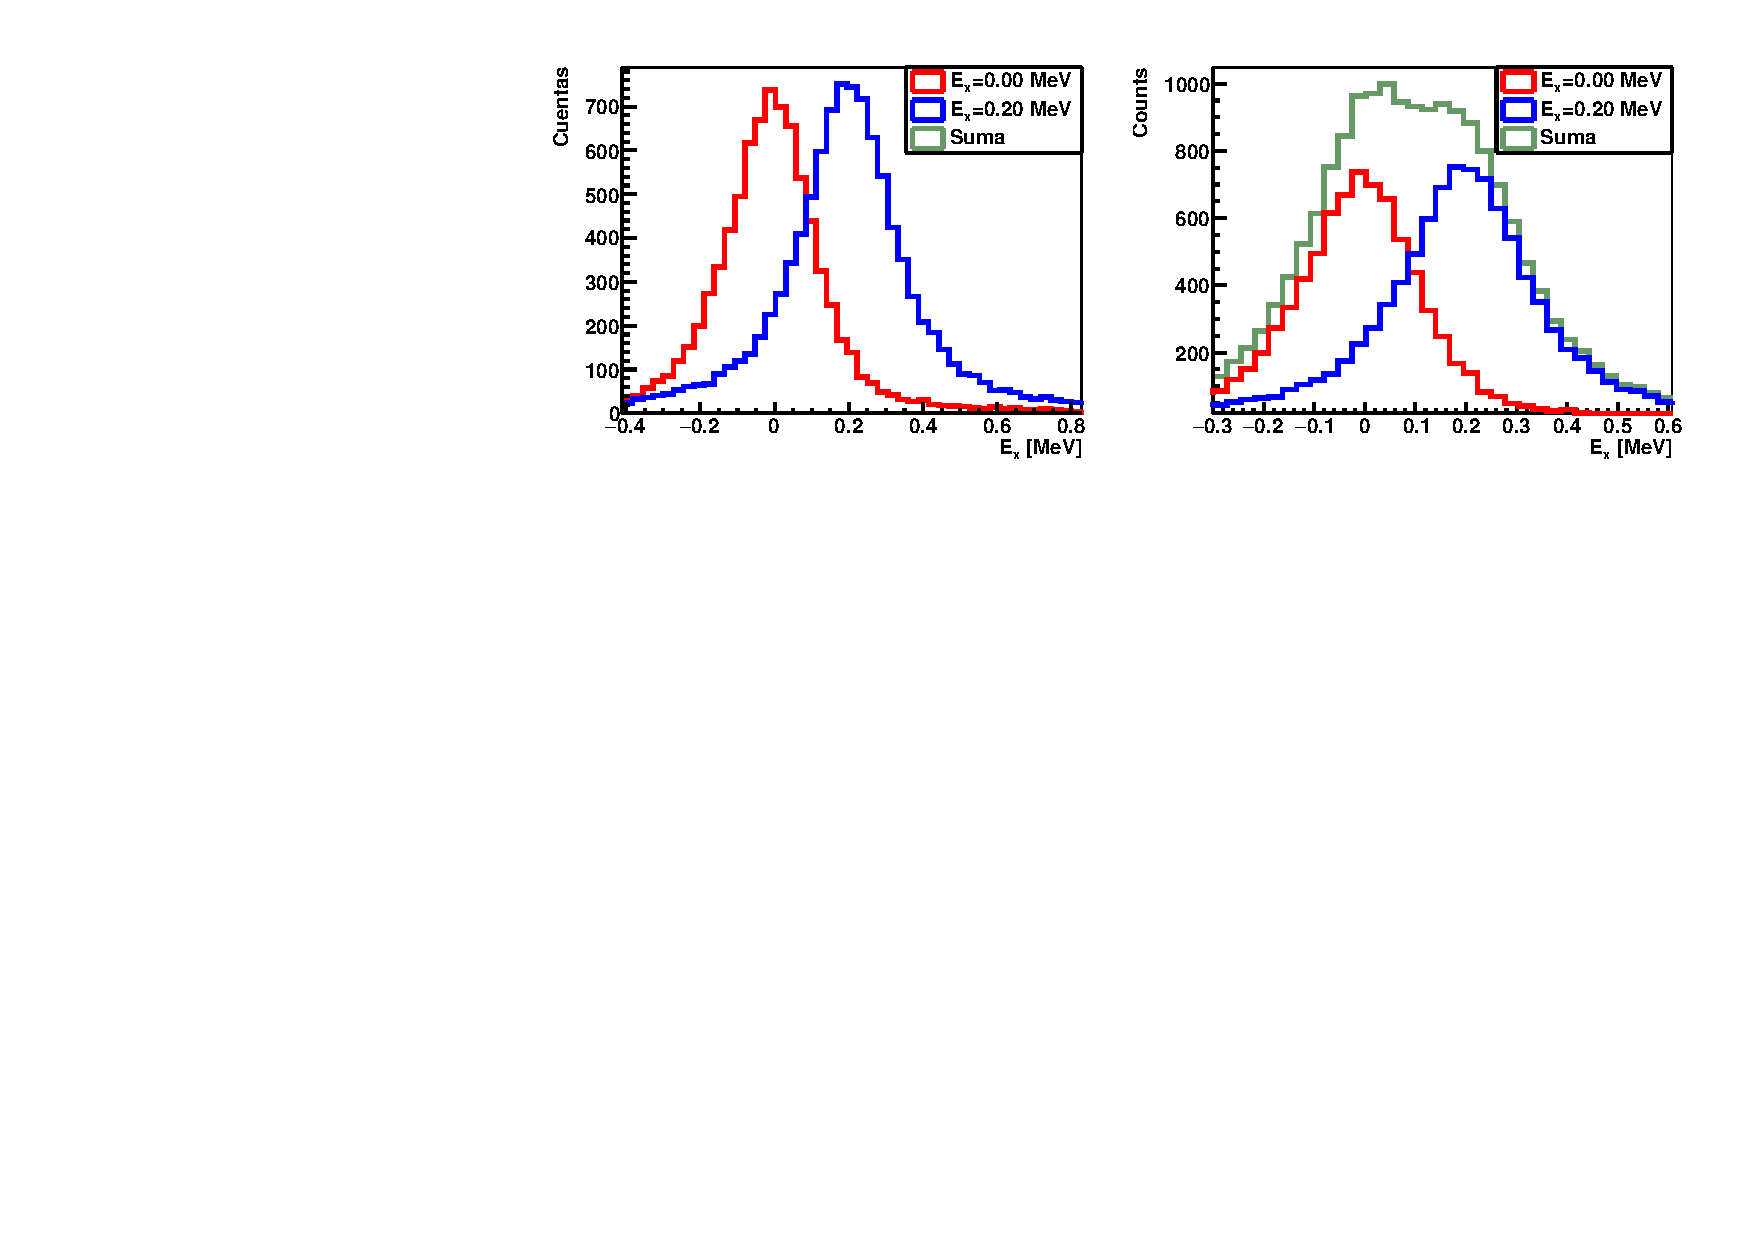
\includegraphics[width=0.9\textwidth]{Imagenes/Rec_incIdx1_single.pdf}
    \caption{Energía de excitación para $\sigma_{str}$.}
    \label{Fig:05-RecExcIdx1}
\end{figure}

\subsection{Recostrucción solo con stragling angular}

Aquí solo vamos a tener en cuenta el efecto de la dispersión angular, con el cual obtenemos una varianza gaussiana tal que: 

\begin{equation}
    \sigma_{\theta}(0.0) = \num{0.201336762255(0.0006744131)} \ \text{MeV} \quad 
    \sigma_{\theta}(0.2) = \num{0.168440735045(0.0007209796)} \ \text{MeV}
\end{equation} 
con un valor mucho mas grande que el anterior y que como podemos ver en \cref{Tab:05-ExcRec} es prácticamente toda la contribución a $\sigma_{tot}$. En la imagen \cref{Fig:05-RecExcIdx2} podemos ver como ya no diferenciamos los picos en el histograma apilado. Sin embargo, debemos tener en cuenta que el número de 

\vspace*{-0.25cm}
\begin{figure}[H]
    \centering
    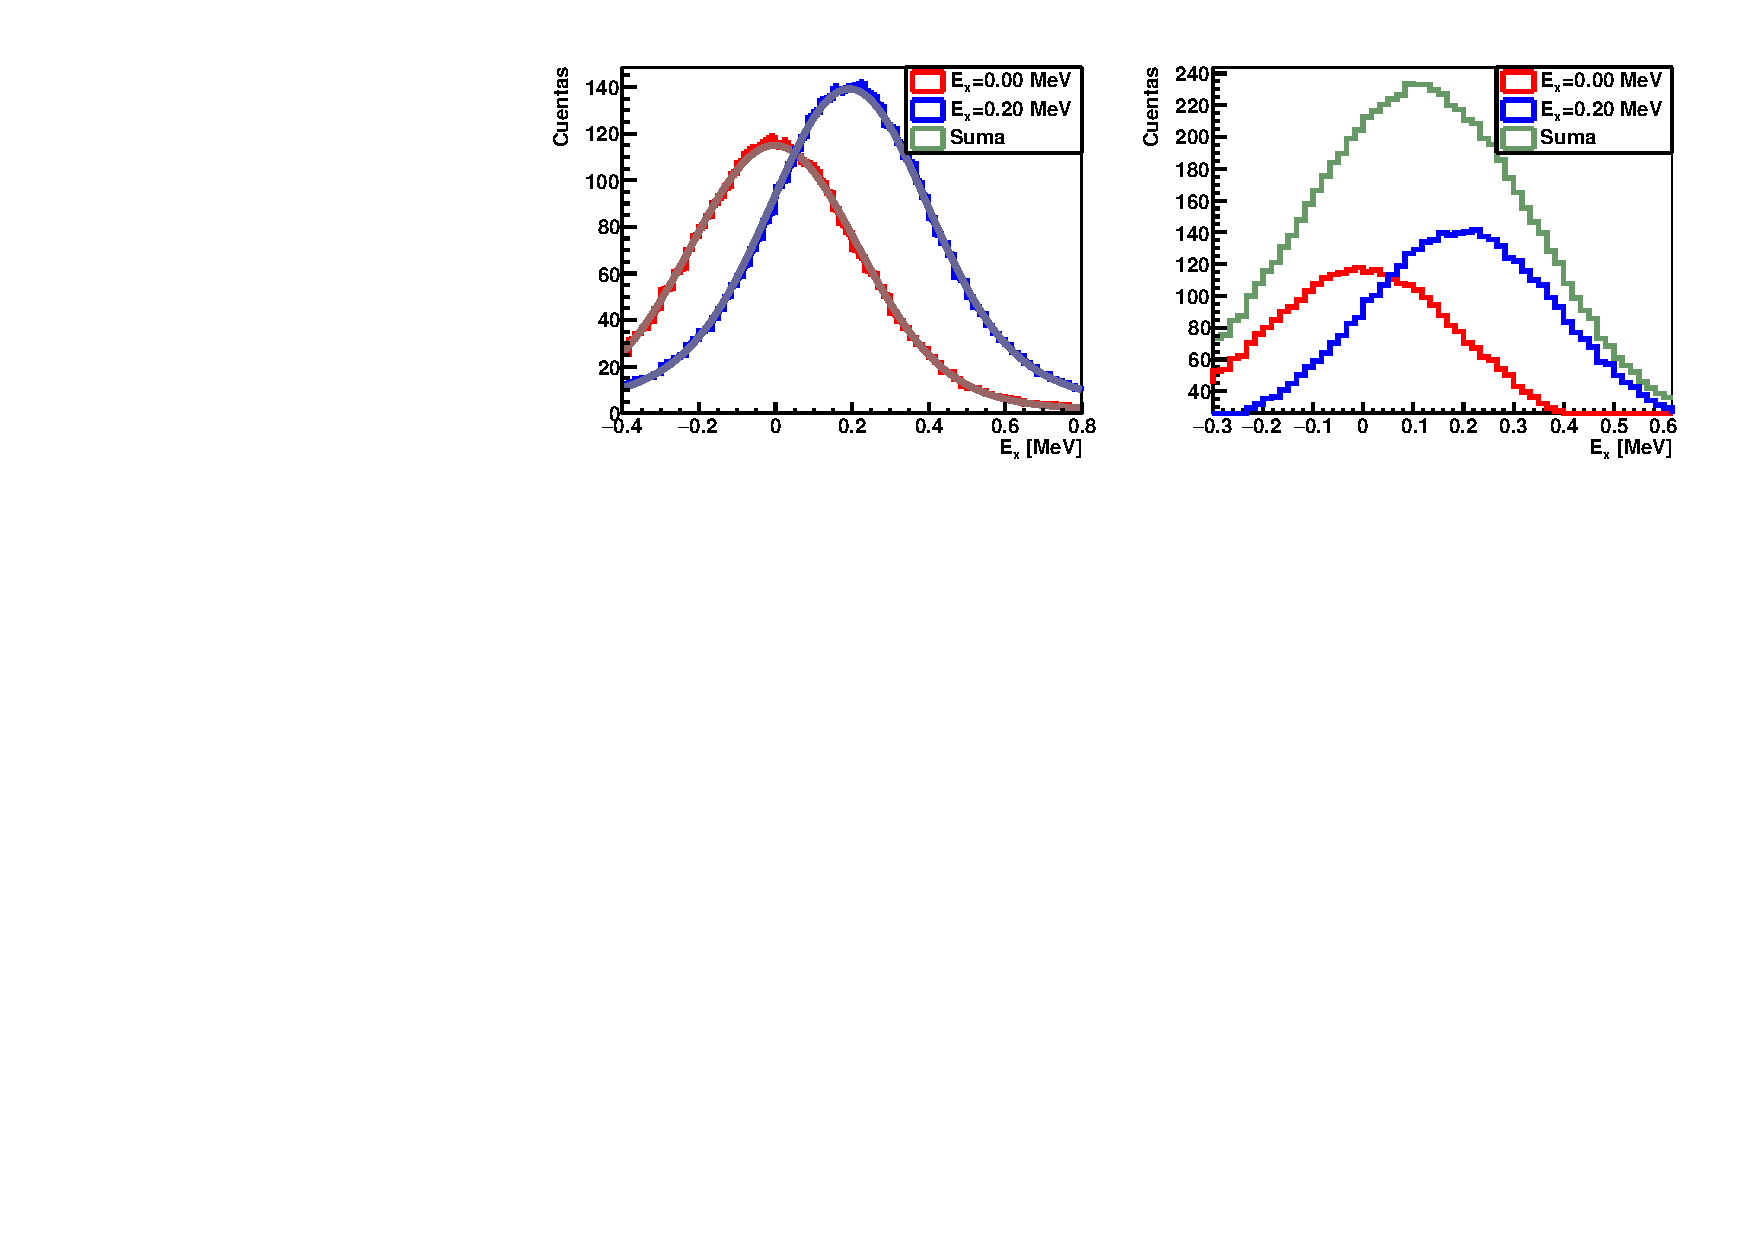
\includegraphics[width=0.9\textwidth]{Imagenes/Rec_incIdx2_single.pdf}
    \caption{Energía de excitación para $\sigma_{\theta}$.}
    \label{Fig:05-RecExcIdx2}
\end{figure}

\subsection{Recostrucción con todas las fuentes de incertidumbre}

Aquí solo vamos a tener en cuenta todos las fuentes de incertidumbre implementadas, obteniendo así: 

\begin{equation}
    \sigma_{tot}(0.0) =\num{0.219033325961(0.0006865088)} \ \text{MeV} \quad 
    \sigma_{tot}(0.2) = \num{0.179463342520(0.0007321261)} \ \text{MeV}
\end{equation} 
e, igual que en el caso anterior, no podemos distiguir los picos del histograma apilado \cref{Fig:05-RecExcIdx0}. 
\vspace*{-0.25cm}
\begin{figure}[H]
    \centering
    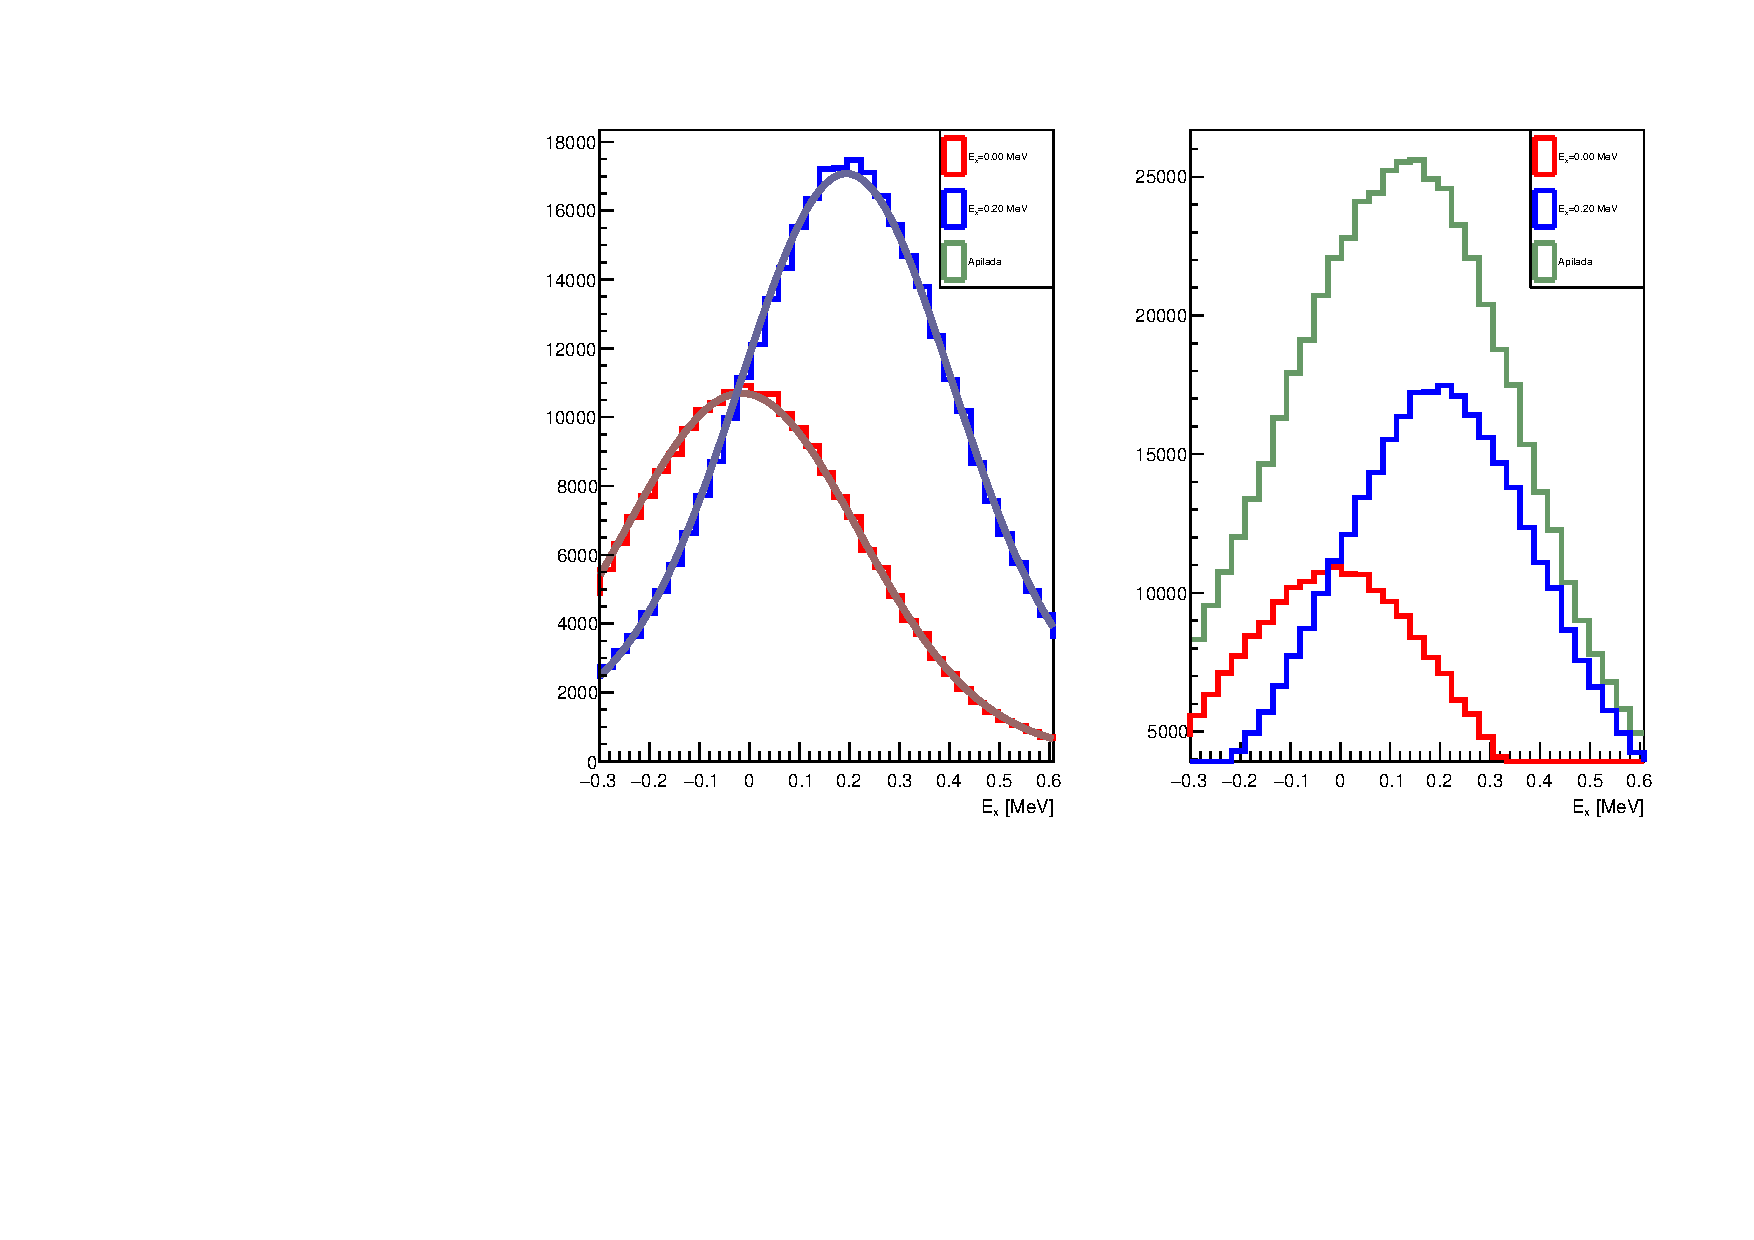
\includegraphics[width=0.9\textwidth]{Imagenes/Rec_incIdx0_single.pdf}
    \caption{Energía de excitación para $\sigma_{tot}$.}
    \label{Fig:05-RecExcIdx0}
\end{figure}


\subsection{Recuperación de eventos a través del trigger}

